\breaksection{Internal elements --- The Circular Economy}\label{sec:quantification_internal_cei}
\subsection{Introduction}

\textbf{Main sources:}~\cite{pardo2018ce,morseletto2020cetargets,eu2018cemonitoring,marino2020ce, oecd2015greengrowth, calistofriant2021ce, stahel2019ce,pbl2021ce, reike2018rex,kirchherr2017circ,nl2023ceplan}

\boxgreen{\textbf{Circular Strategies}}{
        \textbf{Scenario elements}
        \begin{itemize}
          \item \textbf{R0-2:}\\  Refuse, Reduce, Reuse (including 'sharing economy')
          \item \textbf{R3:} \\ Repair
          \item \textbf{R4-5:}\\  Refurbish and Remanufacture
        \end{itemize}
        \textbf{Waste model parameters include:}
        \begin{itemize}
          \item \textbf{Put-on-market:} \\ function of consumer behaviour (internal) 
          \item \textbf{Lifetimes:} \\ function of repair rate, durability, design-for-repair
          \item \textbf{Waste composition:} \\ function of product composition, durability (weight), design-for-repair, etc.
          \item \textbf{Collection rate:} \\ function of consumer engagement in re-X strategies, collection infrastructure, legislation, export rate
        \end{itemize}
        \textbf{Recovery model parameters include:}
        \begin{itemize}
          \item \textbf{Transfer coefficients:} \\ function of design-for-(re-X) strategies, recovery technology (internal)
          \item \textbf{Recovery system size:} \\ function of collection rate
        \end{itemize}
          }
        
\subsubsection{The Circular Economy and its re-X strategies}

The re-X strategies underpin the circular economy, embodying a range of actions and approaches. These strategies are conceptualised in various ways, depending on the focus and perspective of different authors. The description that follows is based on the framework provided by ~\cite{reike2018rex}, with a detailed mapping of these strategies illustrated in Figure~\ref{fig:rex-map}.

\begin{description}
    \item[R0: Refuse] — This concept is applied both in consumer and producer contexts. For consumers, it means choosing not to buy or use products or services that are not needed or are unsustainable, thereby preventing waste creation. For producers, it involves refusing the use of specific hazardous materials and designing production processes to avoid waste. This approach is integral to shifting towards a more post-material lifestyle and reducing packaging waste.

    \item[R1: Reduce] — Reduce is used in a consumer-oriented, producer-oriented, and generic sense. It encompasses using products less frequently, with more care, and for longer, and making repairs for life extension. For producers, it involves using less material per unit of production, a concept known as dematerialization. It also includes participation in the sharing economy through pooling and sharing products.

    \item[R2: Resell/Reuse] — Resell and Reuse involve bringing products back into the economy after initial use, either by reselling or reusing them for the same or a different purpose. This concept includes direct reuse of products such as second-hand sales and reuse in fabrication like refurbishment and remanufacturing. Quality inspections, minor repairs, and online consumer-to-consumer auctions are part of this strategy.

    \item[R3: Repair] — Repair aims to extend the product's lifespan by bringing it back to working order, fixing minor defects, or replacing broken parts. It can be performed by various actors, including the customer, repair companies, or through non-commercial peer-to-peer repair workshops. Planned repairs and ad-hoc repairs are both included under this concept.

    \item[R4: Refurbish] — Refurbishing typically applies to large multi-component products where many components are replaced or repaired, resulting in an overall upgrade of the product. This process brings the product up to a state-of-the-art level using newer, more advanced components, and is often seen in industries like aviation and construction.

    \item[R5: Remanufacture] — Remanufacture involves disassembling, checking, cleaning, and replacing or repairing the full structure of a product in an industrial process. It is distinguished from refurbishing by the extent of disassembly and replacement of components, often resulting in a product that is like new but with a shorter expected lifespan due to the use of recycled components.

    \item[R6: Repurpose] — Repurposing involves adapting discarded goods or components for another function, giving the material a distinct new lifecycle. This can result in both low and high-value end-products and is popular in industrial design and art communities. Examples include transforming defective microchips into jewellery or plastic sheeting into handbags.

    \item[END OF CIRCULAR STRATEGIES] — The following strategies belong to the recovery system

    \item[R7: Recycle Materials] — Recycling involves processing mixed streams of post-consumer products or post-producer waste streams using technological equipment to capture pure materials. It usually results in secondary materials that do not maintain any of the original product structure and can be re-applied anywhere. Recycling typically requires high energy inputs for collection and re-processing.

    \item[R8: Recover (energy)] — Recovery primarily refers to capturing energy embodied in waste, linking it to incineration combined with producing energy, or the use of biomass. It is also used to describe the collection of used products for disassembly, sorting, and cleaning for utilization, and the extraction of elements or materials from end-of-life composites.

    \item[R9: Re-mine] — Re-mining involves the retrieval of materials after the landfilling phase, including extracting valuable parts from disposed products and mining valuable resources stored in old landfills or urban mining. This practice is becoming more lucrative with technological advancements, allowing for the effective extraction of resources from waste stock.
\end{description}

\begin{figure}[h!]
    \centering
    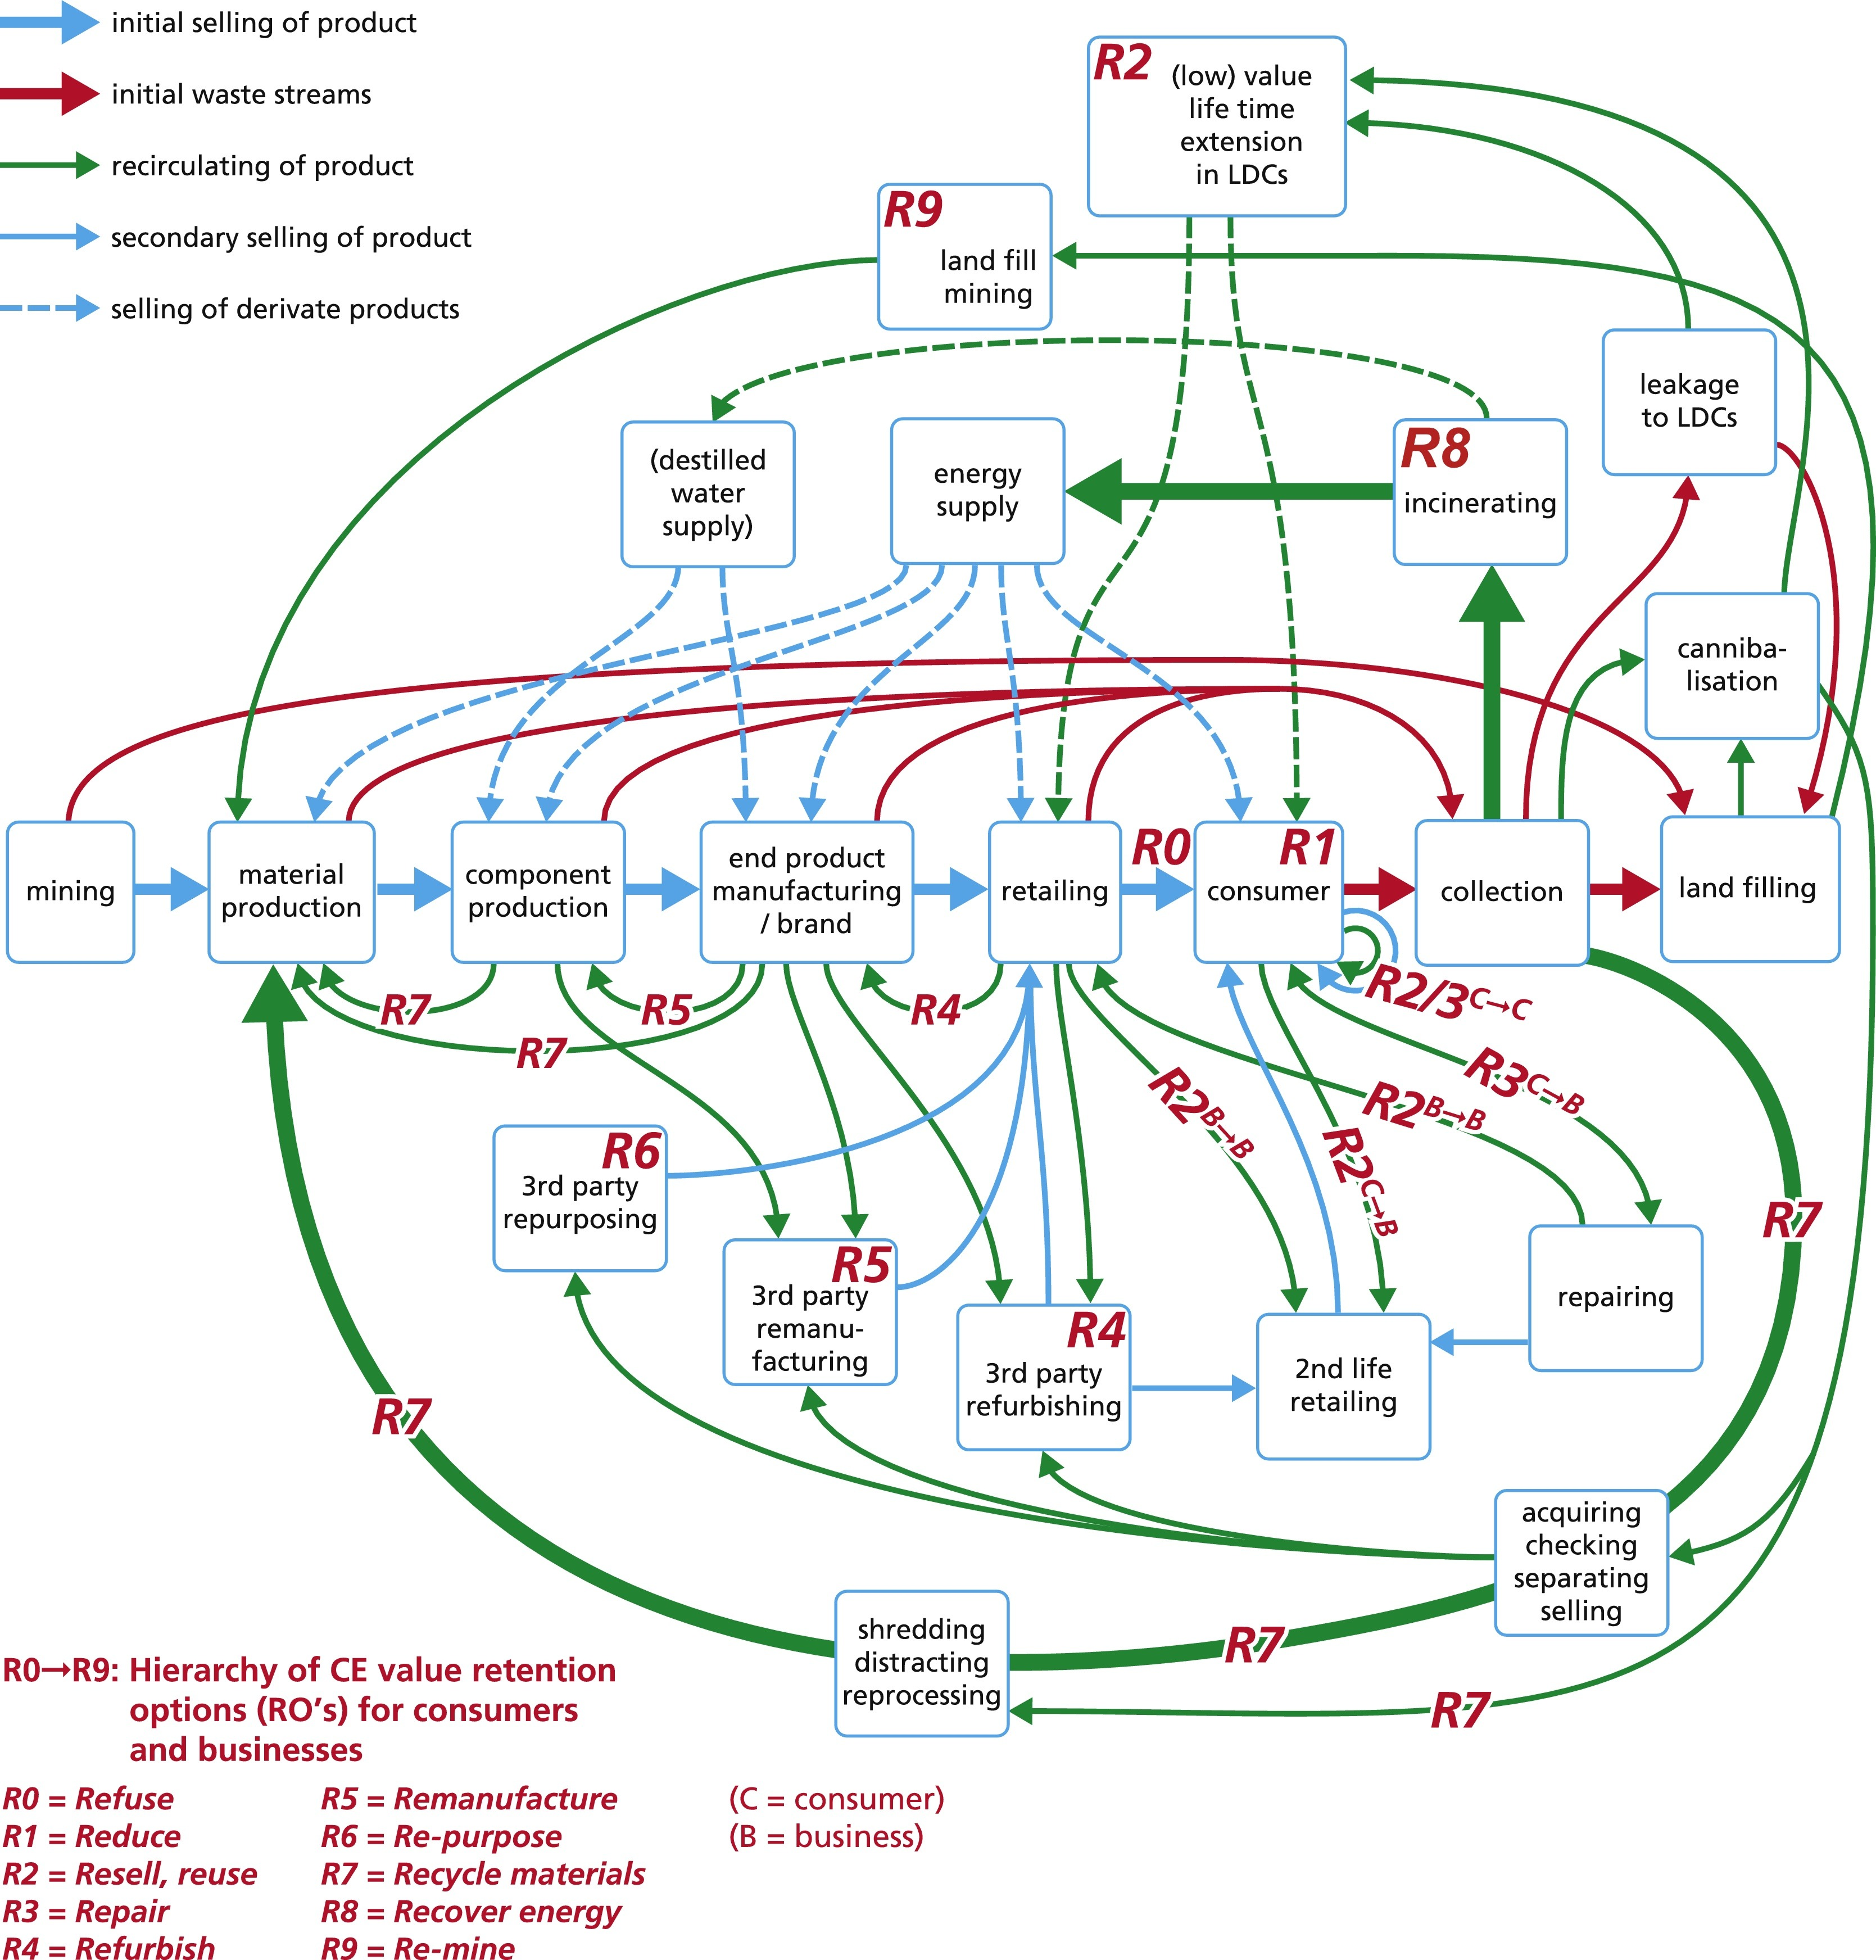
\includegraphics[width=\linewidth]{130quantification/internal/cei/reike2018.jpg}
    \caption[A detailled mapping of the re-X strategies in the circular economy]{A detailled mapping of the re-X strategies in the circular economy~\cite{reike2018rex}}
    \label{fig:rex-map}
\end{figure}
\FloatBarrier

\subsubsubsection{EU Circular Economy Indicators (CEIs)}

See the EU working documents~\cite{eu2018cemonitoring} and~\cite{eu2023cemonitoring} for more detailled assssment of progress relating to the CEIs. \autoref{tab:eu2023ceprogress} presents an overview of the EU's CEIs including their target for 2023.

\begin{table}[h!]
  \centering
  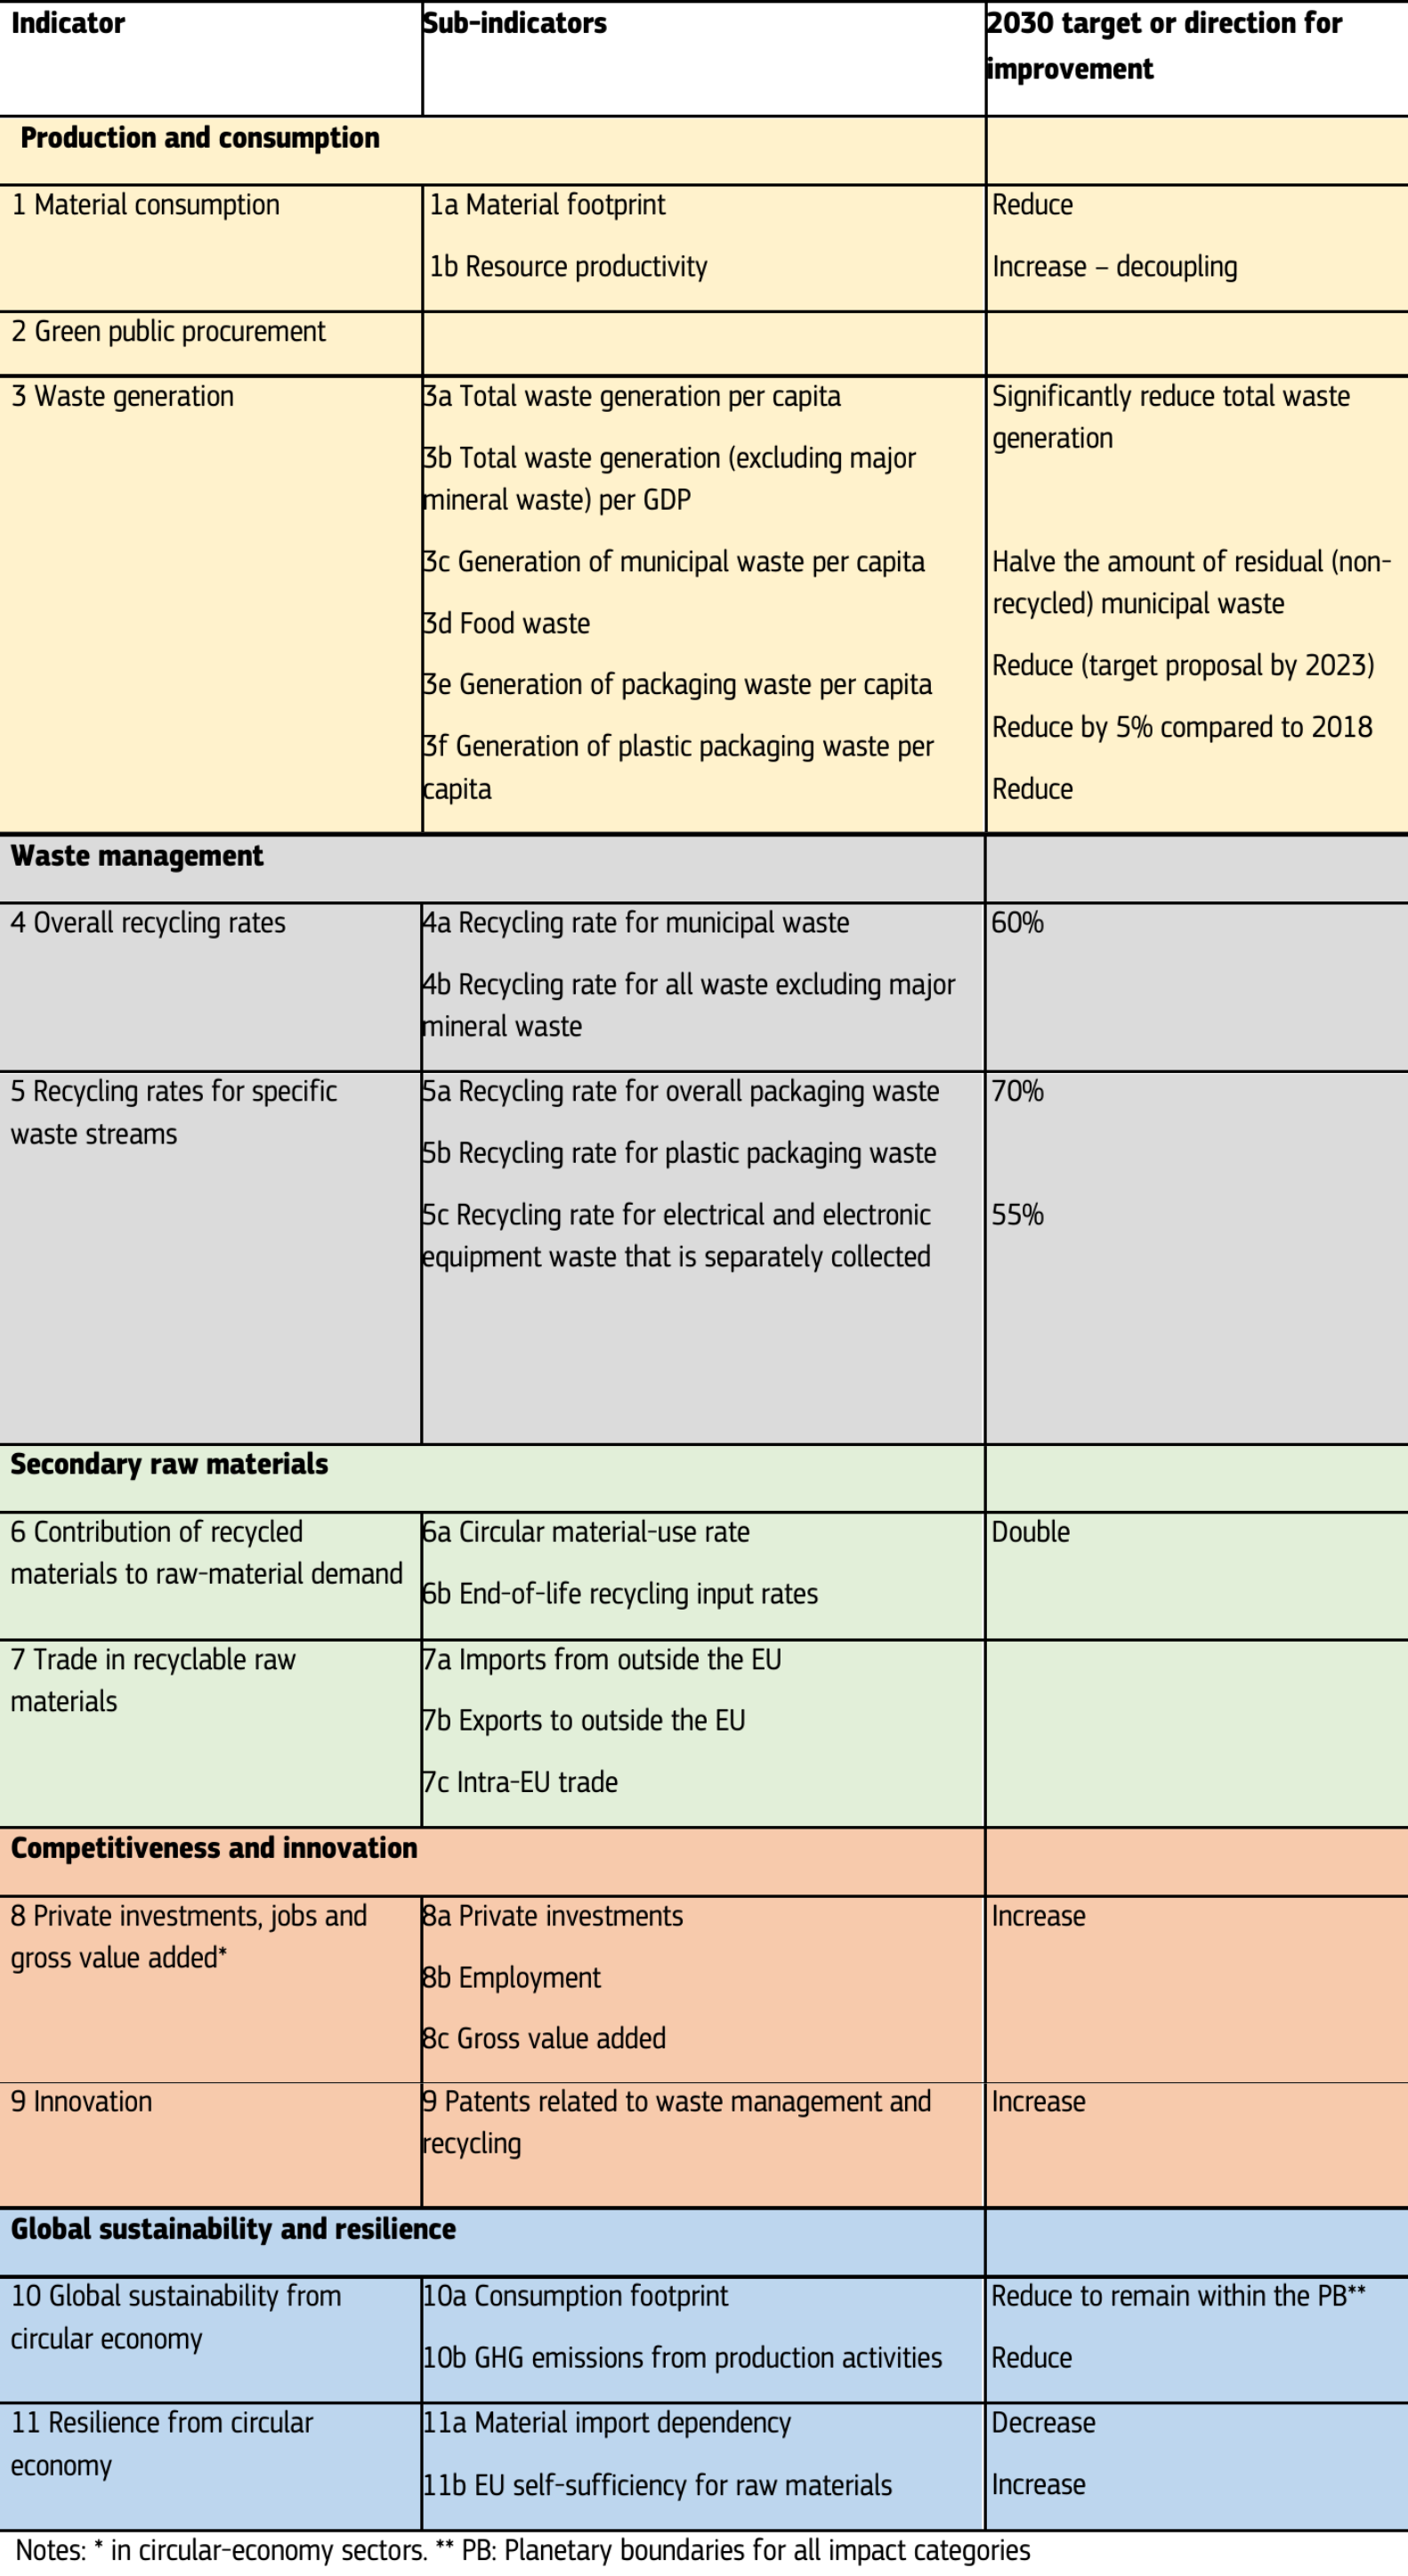
\includegraphics[height=0.9\textheight]{130quantification/internal/cei/eu2023ceprogress.png}
  \caption[EU Circular Economy Indicators (CEIs) and their targets for 2023]{EU Circular Economy Indicators (CEIs) and their targets for 2023~\cite{eu2023cemonitoring}}
  \label{tab:eu2023ceprogress}
\end{table}

\autoref{tab:cei} lists the relevant EU circular indicators (CEIs) along with their significance for FutuRaM's models and their changes between 2000--2022.

\begin{landscape}
    \centering
    \small
    \begin{longtable}{|C{2.5cm}|L{7cm}|C{6cm}|C{6cm}|C{1.5cm}|}
    \caption{EU circular indicators (CEIs) and their significance for FutuRaM's models}\label{tab:cei}\\
          \hline
          \rowcolor{headerblue} % Applying the header color
          \textcolor{white}{\textbf{CODE}} & \textcolor{white}{\textbf{TITLE}} & \textcolor{white}{\textbf{WS MODEL RELEVANCE}} & \textcolor{white}{\textbf{RECOVERY MODEL RELEVANCE}} & \textcolor{white}{\textbf{RATIO 2022:2000}} \\
          \hline
          \endfirsthead%
          \hline
          \multicolumn{5}{r}{\textcolor{headerblue}{\textit{{Continued on next page}}}} \\
          \endfoot%
          \rowcolor{white}
          \multicolumn{5}{c}{{\textcolor{headerblue}{\textit{\tablename\ \thetable{} --- Continued from previous page}}}} \\
          \hline
          \rowcolor{headerblue} % Applying the header color       
          \textcolor{white}{\textbf{CODE}} & \textcolor{white}{\textbf{TITLE}} & \textcolor{white}{\textbf{WS MODEL RELEVANCE}} & \textcolor{white}{\textbf{RECOVERY MODEL RELEVANCE}} & \textcolor{white}{\textbf{RATIO 2022:2000}} \\ \hline
          \endhead%
          \bottomrule
          \endlastfoot%
      \csvreader[late after last line=\ , separator=semicolon]{csvs/cei_eu.csv}{}{
        \csvcoli& \csvcolii& \csvcoliii& \csvcoliv& \csvcolv \\
      } \\
      \bottomrule
    \end{longtable}
  \end{landscape}


\autoref{fig:cei} depicts the CEIs, their trends from 2000-2022, and their linear forecasts until 2050. An interactive figure can be viewed \href{https://futuram-project.github.io/FutuRaM.github.io/WP2/assets.html}{here~\faLink}. Note that the linear trends are not deemed to be representative of the actual future values, but are used to illustrate the trends and the magnitude of the changes. There will be constraints defined to limit and shape the growth of the CEIs in each of the scenarios. The settings for this will be determined from the waste stream quantification and the scenario storylines.

\begin{landscape}
    \begin{figure}[h!]
        \centering
        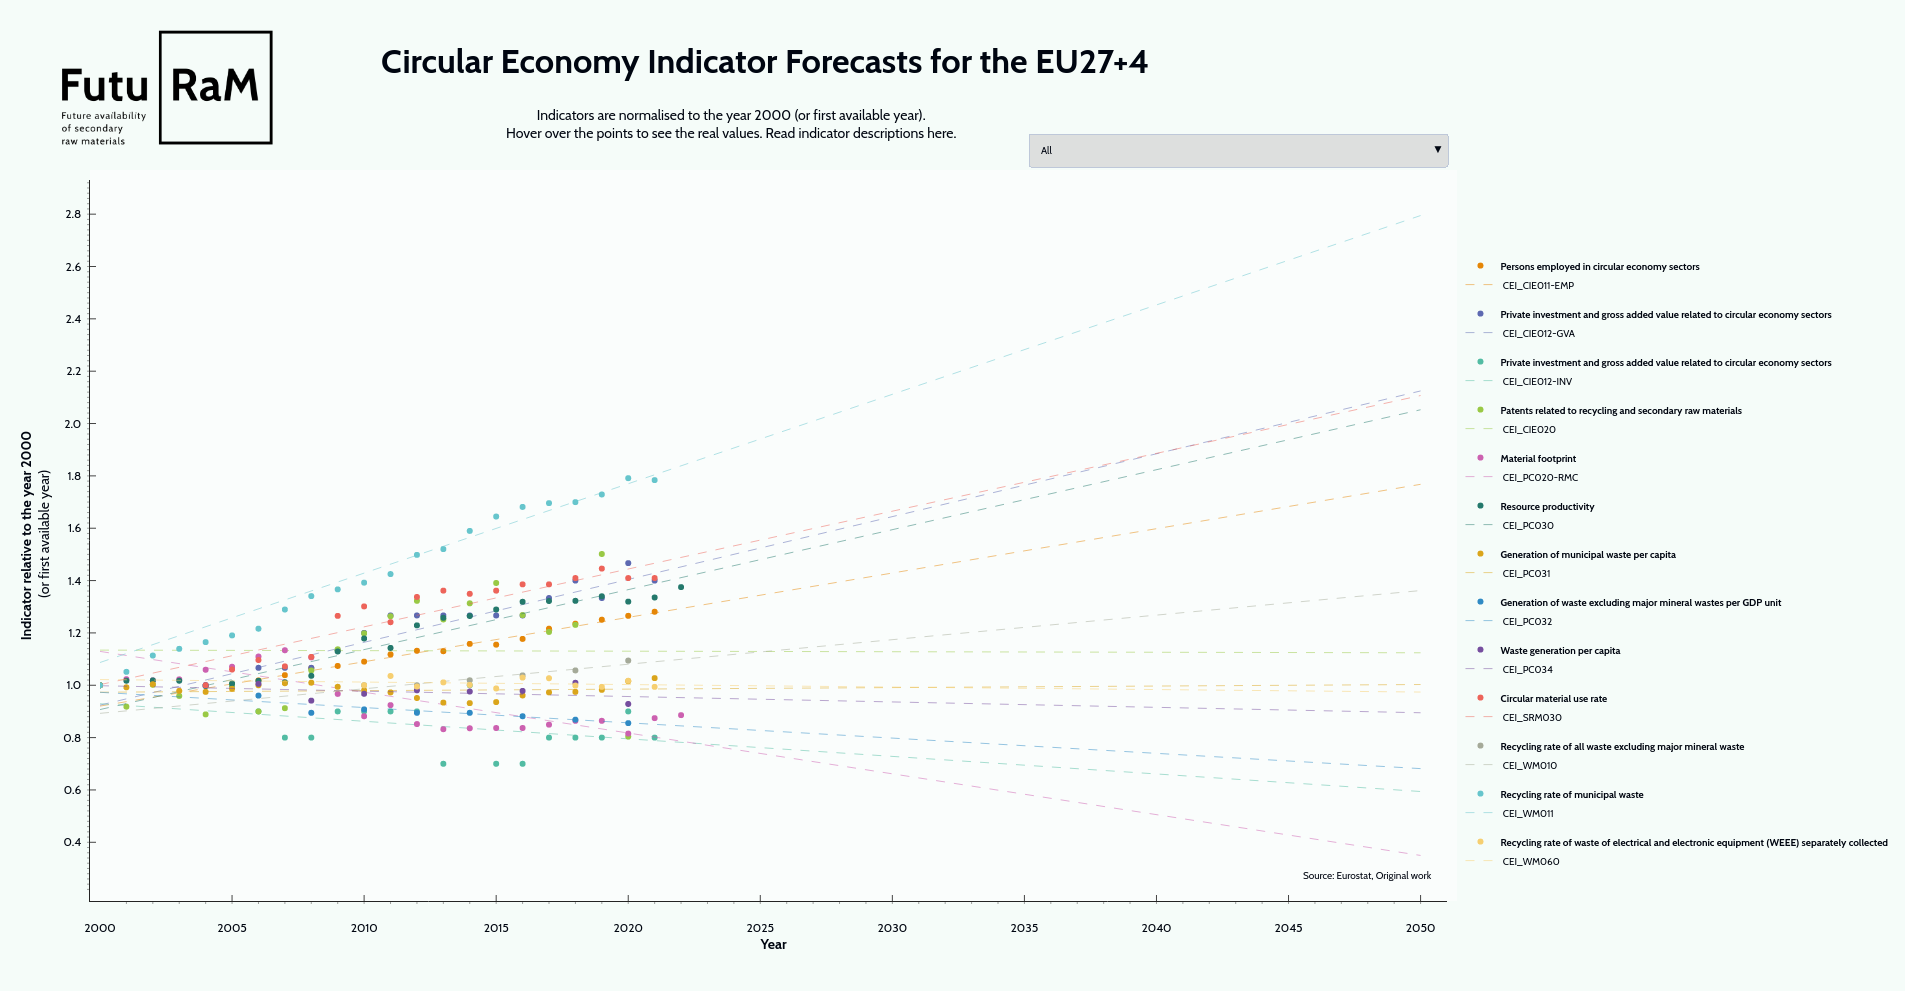
\includegraphics[width=1\linewidth]{130quantification/internal/cei/cei_eu.png}
        \caption{EU Circular Economy Indicators (CEIs) - trends from 2000-2022 and linear forecasts}
        \label{fig:cei}
    \end{figure}
\end{landscape}
    



\subsectionEndline
\clearpage

\subsection{Summary}


The environmental and socio-economic impacts of raw material use are most effectively addressed at the product group level. Examining a product group as a whole, rather than focusing on individual resources or materials, allows for a comprehensive understanding and management of its utilisation and the environmental impacts across the production chain and product lifecycle~\cite{pbl2021ce}. 

Additionally, setting impact targets for product groups aligns more closely with the capacity of stakeholders within the chain to modify resource usage or mitigate related environmental impacts.

Although the nature and magnitude of raw material use impacts can differ significantly among product groups, necessitating tailored impact targets, there is also a need for simplicity in target setting. A manageable and communicable approach for governments is to aim for a significant reduction, such as halving the environmental impact at the product group level. 

The benefit of establishing more general effect targets lies in the flexibility it offers for varying focuses across different product groups. A target set at the product group level is not only clear and easily communicable but also acknowledges the complexity and diversity inherent in a circular economy.


\boxreview{This section will be completed once the individual waste stream sections for each parameter are complete.}
\clearpage

% pull in the other subsections

\subsection{The EU Circular Economy Indicators: \textit{Description}}

\textbf{Main sources:}~\cite{eu2018cemonitoring,eurostat2023data,eu2023cemonitoring}


\boxparameter{The EU Circular Economy Indicators}{Stable}{Strong increase in recycling and recovery related indicators}{Strong in circularity related indicators}

\subsubsection{Economic Indicators}

\subsubsubsection{CEI\_CIE011:\\ Persons employed in circular economy sectors \& \\ CEI\_CIE012:\\ Private investment and gross added value related to circular economy sectors} 
\textbf{Indicator metadata:}   \href{https://ec.europa.eu/eurostat/cache/metadata/en/cei_cie011_esmsip2.htm}{\faExternalLink}

{\large\textbf{Context:}}  \\ \indent
Targets economic activities that contribute to the circular economy, delineating those activities through established environmental policy frameworks and classifications.

{\large\textbf{Indicator Description:}}  \\ \indent
The indicator encompasses ``Private investments'', ``Persons employed'' and ``Gross value added''. Eurostat has developed a method to derive these key economic variables, incorporating a multi-step approach: establishing a conceptual framework based on international environmental policy definitions, mapping and classifying relevant activities against an integrated system of economic classifications (using NACE, CPA, and PRODCOM codes), and finally compiling data using defined estimation procedures. The primary outputs of this process are the measurements of employment in FTE, gross value added at factor cost, and investments in tangible goods, each quantified in million euros.

{\large\textbf{Unit:}}  \\ \indent
Economic metrics are presented in million euros, with employment figures given in full-time equivalents (FTE); both sets of figures are also contextualised as percentages of GDP and total employment, respectively.

{\large\textbf{Source Data:}}  \\ \indent
Data is sourced from a combination of Structural Business Statistics, National Accounts, Prodcom surveys, and the Labour Force Survey, enriched by additional sector-specific statistics.

\subsubsubsection{CEI\_CIE020: Patents related to recycling and secondary raw materials}
\textbf{Indicator metadata:}   \href{https://ec.europa.eu/eurostat/cache/metadata/en/cei_cie020_esmsip2.htm}{\faExternalLink}

{\large\textbf{Context:}}  \\ \indent
This indicator is integral to the Circular Economy set, focusing on `competitiveness and innovation' and serving to gauge progress towards a more circular economy.

{\large\textbf{Indicator Description:}}  \\ \indent
The indicator enumerates the number of patent families pertinent to recycling and secondary raw materials, leveraging the Cooperative Patent Classification to ensure unique counts.

{\large\textbf{Unit:}}  \\ \indent
The unit of measure is the number of patent families, with a secondary metric of patents per million inhabitants.

{\large\textbf{Source Data:}}  \\ \indent
Sourced from the European Patent Office (EPO), the data are extracted and analyzed by the Joint Research Centre (JRC), using the PATSTAT database.

\subsubsubsection{CEI\_PC030: Resource productivity}
\textbf{Indicator metadata:}   \href{https://ec.europa.eu/eurostat/cache/metadata/en/cei_pc030_esmsip2.htm}{\faExternalLink}

{\large\textbf{Context:}} \\
Embedded within the Circular Economy indicator suite, this metric tracks progress in `Production and consumption', emphasizing material use efficiency to gauge economic growth relative to resource use.

{\large\textbf{Indicator Description:}}  \\ \indent
Resource productivity is articulated as GDP over DMC, showcasing the efficiency of material utilization within an economy. This indicator assists in understanding the dynamics between economic performance and environmental pressure.

{\large\textbf{Unit:}}  \\ \indent
Measured in three distinct units: euro per kg in chain-linked volumes (2015), PPS per kg, and as an index (2000=100) for temporal and spatial comparisons.

{\large\textbf{Source Data:}}  \\ \indent
The European Statistical System (ESS) supplies the data, with Eurostat disseminating information on DMC and GDP, derived from the Material Flow Accounts and GDP and main components datasets, respectively.

\subsubsection{Waste and Material Indicators}

\subsubsubsection{CEI\_PC020: Material footprint}
\textbf{Indicator metadata:}   \href{https://ec.europa.eu/eurostat/cache/metadata/en/cei_pc020_esmsip2.htm}{\faExternalLink}

{\large\textbf{Context:}}  \\ \indent
The `Material footprint' indicator is a critical component of the Circular Economy monitoring framework, highlighting the `production and consumption' thematic area. It reflects the EU's impact on global resources, pertinent to the EU's consumption exceeding its production, especially concerning goods manufactured in Asia and consumed in Europe.

{\large\textbf{Indicator Description:}}  \\ \indent
This indicator assesses the global demand for material extraction driven by EU consumption and investment. The Material Footprint provides insight into the environmental burden shifted to other regions due to the EU`s consumption patterns. It is expressed through the Raw Material Consumption (RMC) metric, indicating the material extraction required for goods consumed within the EU.

{\large\textbf{Unit:}}  \\ \indent
The unit of measure is tonnes per capita.

{\large\textbf{Source Data:}}  \\ \indent
Data source: European Statistical System (ESS)
Data provider: Statistical Office of the European Union (Eurostat).
Material flow accounts in raw material equivalents -- modelling estimates (env\_ac\_rme).~\href{https://ec.europa.eu/eurostat/web/products-datasets/-/env_ac_rmefd}{\faExternalLink}
Material flow accounts in raw material equivalents by final uses of products - modelling estimates (env\_ac\_rmefd).~\href{https://ec.europa.eu/eurostat/web/products-datasets/-/env_ac_rmefd}{\faExternalLink}

\subsubsubsection{CEI\_PC031: Generation of municipal waste per capita}
\textbf{Indicator metadata:}   \href{https://ec.europa.eu/eurostat/cache/metadata/en/cei_pc031_esmsip2.htm}{\faExternalLink}

{\large\textbf{Context:}}  \\ \indent
The `Generation of municipal waste per capita' indicator is integral to the Circular Economy indicator set, falling under the `production and consumption' thematic area. It underscores efforts to sustain product and material value in the economy, minimize waste generation, and drive waste prevention strategies in alignment with the Waste Hierarchy.

{\large\textbf{Indicator Description:}}  \\ \indent
This indicator tracks municipal waste generated and managed by local authorities or entities appointed by them. It predominantly accounts for household waste, although it may include waste from commercial activities, offices, and public institutions, reflecting consumer behaviour and the impact of waste reduction measures.

{\large\textbf{Unit:}}  \\ \indent
The unit of measure is kilograms per capita, based on the annual average population.

{\large\textbf{Source Data:}}  \\ \indent
The data is provided by Eurostat, consistent with the high-quality standards of the European Statistical System (ESS), deriving from the Municipal waste by waste operations report, collected under the OECD/Eurostat Joint Questionnaire. Data submission is voluntary, known as a `gentlemen's agreement'.

\subsubsubsection{CEI\_PC032: \\Generation of waste excluding major mineral wastes per GDP unit}
\textbf{Indicator metadata:}   \href{https://ec.europa.eu/eurostat/cache/metadata/en/cei_pc032_esmsip2.htm}{\faExternalLink}

{\large\textbf{Context:}}  \\ \indent
The `Generation of municipal waste per capita' indicator is integral to the Circular Economy indicator set, falling under the `production and consumption' thematic area. It underscores efforts to sustain product and material value in the economy, minimize waste generation, and drive waste prevention strategies in alignment with the Waste Hierarchy.

{\large\textbf{Indicator Description:}}  \\ \indent
This indicator tracks municipal waste generated and managed by local authorities or entities appointed by them. It predominantly accounts for household waste, although it may include waste from commercial activities, offices, and public institutions, reflecting consumer behaviour and the impact of waste reduction measures.

{\large\textbf{Unit:}}  \\ \indent
The unit of measure is kilograms per capita, based on the annual average population.

{\large\textbf{Source Data:}}  \\ \indent
The data is provided by Eurostat, consistent with the high-quality standards of the European Statistical System (ESS), deriving from the Municipal waste by waste operations report, collected under the OECD/Eurostat Joint Questionnaire. Data submission is voluntary, known as a gentlemen's agreement.

\subsubsubsection{CEI\_PC034: Waste generation per capita}
\textbf{Indicator metadata:}   \href{https://ec.europa.eu/eurostat/cache/metadata/en/cei_pc034_esmsip2.htm}{\faExternalLink}

{\large\textbf{Context:}}  \\ \indent
The `Waste generation per capita' indicator is a key component of the Circular Economy monitoring framework, aimed at assessing the effectiveness of EU policies focused on waste reduction and resource efficiency within the `production and consumption' thematic area.

{\large\textbf{Indicator Description:}}  \\ \indent
This indicator reflects the total waste generation within a country, including major mineral wastes from all economic activities and households. It is an essential measure for evaluating the impact of waste prevention measures, allowing comparison of Member States' performance over time.

{\large\textbf{Unit:}}  \\ \indent
The unit of measure is kilogram per capita

{\large\textbf{Source Data:}}  \\ \indent
The data originates from the European Statistical System (ESS), specifically Eurostat, which collates information reported by countries under the Waste Statistics Regulation (EC) No 2150/2002.

\subsubsubsection{CEI\_SRM030: Circular material use rate}
\textbf{Indicator metadata:}   \href{https://ec.europa.eu/eurostat/cache/metadata/en/cei_srm030_esmsip2.htm}{\faExternalLink}

{\large\textbf{Context:}}  \\ \indent
As a core metric within the Circular Economy indicator set, the `Circular material use rate' is crucial for monitoring advancements in the utilization of `secondary raw materials'. It encapsulates the circular economy's goal to enhance material recycling, reduce waste, and curb the reliance on primary raw material extraction.

{\large\textbf{Indicator Description:}}  \\ \indent
This indicator assesses the proportion of recycled material re-entering the economy against the overall material consumption, serving as a benchmark for the `circularity rate'. It signifies the efficiency of resource use by contrasting the circular use of materials against the aggregate domestic material consumption (DMC), adjusted for waste trade.

{\large\textbf{Unit:}}  \\ \indent
The indicator is presented as a percentage, depicting the share of recycled material in total material usage, reflecting the level at which secondary materials replace primary resources.

{\large\textbf{Source Data:}}  \\ \indent
Data is sourced from the European Statistical System (ESS) and Eurostat, employing a trio of statistical resources: waste treatment statistics, material flow accounts, and international trade data.

\subsubsubsection{CEI\_WM010: Recycling rate of all waste excluding major mineral waste}
\textbf{Indicator metadata:}   \href{https://ec.europa.eu/eurostat/cache/metadata/en/cei_wm010_esmsip2.htm}{\faExternalLink}

{\large\textbf{Context:}}  \\ \indent
This indicator is pivotal for measuring advancements in `waste management`. It gauges the efficiency of resource use by monitoring the volume of materials recycled and reincorporated into the economy, thus encapsulating the essence of material conservation and loss reduction.

{\large\textbf{Indicator Description:}}  \\ \indent
The recycling rate is formulated by the proportion of waste recycled versus the total waste treated, excluding significant mineral waste, rendered in percentage terms. It encompasses both hazardous and non-hazardous waste across all sectors, including household and secondary waste from waste treatment processes, thereby providing a comprehensive snapshot of the national recycling efforts.

{\large\textbf{Unit:}}  \\ \indent
Expressed in percentage

{\large\textbf{Source Data:}}  \\ \indent
Eurostat, under the aegis of the ESS, supplies this data. It incorporates waste treatment information aligned with the Waste Statistics Regulation, fine-tuned with international trade data, to accurately reflect the recycling of domestically produced waste.

\subsubsubsection{CEI\_WM011: Recycling rate of municipal waste}
\textbf{Indicator metadata:}   \href{https://ec.europa.eu/eurostat/cache/metadata/en/cei_wm011_esmsip2.htm}{\faExternalLink}

{\large\textbf{Context:}}  \\ \indent
As an integral part of the Circular Economy indicators, this measure serves as a barometer for the progression towards a more circular economy, with a focus on `waste management`. It assesses the re-utilisation of consumer waste in the economy, capturing the complexities inherent in the diverse composition of municipal waste.

{\large\textbf{Indicator Description:}}  \\ \indent
This indicator quantifies the proportion of municipal waste that is recycled, relative to the total amount of municipal waste produced, presented as a percentage. The breadth of municipal waste includes household refuse and similar commercial and public waste, representing a snapshot of the waste management quality from a consumer perspective.

\textit{"In order to comply with the objectives of this Directive, and move to a European circular economy with a high level of resource efficiency, Member States shall take the necessary measures designed to achieve the following targets: (a) by 2020, the preparing for re-use and the recycling of waste materials such as at least paper, metal, plastic and glass from households and possibly from other origins as far as these waste streams are similar to waste from households, shall be increased to a minimum of overall 50 \% by weight;"} --- Article 11.2 of the Waste Framework Directive.~\cite{eu2008wastedirective}

{\large\textbf{Unit:}}  \\ \indent
The metric of evaluation is a percentage

{\large\textbf{Source Data:}}  \\ \indent
Data source: European Statistical System (ESS)
Data provider: Statistical Office of the European Union (Eurostat) based on data reported by the countries: Municipal waste by waste operations \href{http://ec.europa.eu/eurostat/web/products-datasets/-/env_wasmun}{\faExternalLink} collected via a subset of the OECD/Eurostat Joint Questionnaire, section waste. Data are provided under a so-called gentlemen's agreement.

\subsubsubsection{CEI\_WM060: Recycling rate of waste of electrical and electronic equipment (WEEE) separately collected}
\textbf{Indicator metadata:}   \href{https://ec.europa.eu/eurostat/cache/metadata/en/cei_wm060_esmsip2.htm}{\faExternalLink}

{\large\textbf{Context:}}  \\ \indent
This indicator is a crucial component of the Circular Economy suite, offering insights into the progression towards enhanced sustainability in `waste management'. WEEE, or e-waste, is a rapidly expanding waste stream within the EU that encapsulates items like computers, TVs, refrigerators, and mobile phones. Given the valuable materials found in e-waste, improving recycling processes is of paramount importance.

{\large\textbf{Indicator Description:}}  \\ \indent
The indicator measures the efficiency of WEEE recycling by calculating the ratio of the weight of WEEE processed for recycling/re-use against the total weight of WEEE collected separately, in compliance with Article 11(2) of the WEEE Directive 2012/19/EU~\cite{eu2012weee, eu2012weeerecast}. The indicator's transition from `Recycling rate of e-waste' to its current form is to align more closely with the CE monitoring framework revisions.

The applicability of Directive 2012/19/EU is twofold:
\begin{itemize}
  \item Applicable up to the year 2018 for EEE classified under 10 product categories
        as outlined in Annex I of the Directive, with Annex II providing a
        corresponding indicative product list.
  \item Applicable from the year 2019 forward, where all EEE will be classified within
        6 product categories as delineated in Annex III.
\end{itemize}

{\large\textbf{Unit:}}  \\ \indent
The percentage serves as the unit of measure

{\large\textbf{Source Data:}}  \\ \indent \indent
Data procurement is executed by the ESS and supplied by Eurostat. The indicator's underlying data stems from:
\begin{itemize}
  \item For WEEE by waste operations:
        (env\_waselee)~\href{http://ec.europa.eu/eurostat/web/products-datasets/-/env_waselee}{\faExternalLink}.
  \item For WEEE by waste management operations - open scope, 6 product categories
        (from 2018 onwards):
        (env\_waseleeos)~\href{https://ec.europa.eu/eurostat/web/products-datasets/-/env_waseleeos}{\faExternalLink}.
\end{itemize}


\sectionEndlines
\clearpage

\clearpage
\subsection{The EU Circular Economy Indicators: \textit{Scenarios}}\label{subsec:cei-scenarios}

\boxws{This section will be filled out with the details of exactly how this parameter is incorporated into your stock and flow models}

\subsubsection{Summary}

\boxreview{This summary will be compiled once the individual waste stream sections for each parameter are complete.}

\clearpage

\subsubsection[Scenario I: Business-as-usual]{\iconBAU Scenario I: Business-as-usual}

xx \\


\wasteSubsubsubsecBATT

\wasteSubsubsubsecCDW

\wasteSubsubsubsecELV

\wasteSubsubsubsecMIN

\wasteSubsubsubsecSLASH

\wasteSubsubsubsecWEEE

\subsectionEndline
\clearpage

\subsubsection[Scenario II: Recovery]{\iconREC Scenario II: Recovery}

xx \\


\wasteSubsubsubsecBATT

\wasteSubsubsubsecCDW

\wasteSubsubsubsecELV

\wasteSubsubsubsecMIN

\wasteSubsubsubsecSLASH

\wasteSubsubsubsecWEEE

\subsectionEndline
\clearpage


\subsubsection[Scenario III: Circularity]{\iconCIR Scenario III: Circularity}

xx \\


\wasteSubsubsubsecBATT

\wasteSubsubsubsecCDW

\wasteSubsubsubsecELV

\wasteSubsubsubsecMIN

\wasteSubsubsubsecSLASH

\wasteSubsubsubsecWEEE

\sectionEndlines
\clearpage
\clearpage

\subsection{Refuse, Reduce, Reuse: \textit{Description}}

Refuse, Reduce, and Reuse are the first three short loops (R0-2) in the circular economy scheme. They exist close to the 
consumer and can be linked to commercial or non-commercial actors engaged in extending the product's lifespan~\cite{vermeulen2019rex}.

\boxparameter{Refuse, reduce, reuse}{Stable}{Stable}{Strong increase}


These strategies are pivotal in the circular economy, effectively reducing the environmental impact of products or services.

\begin{itemize}
    \item \textbf{R0 --- Refuse:} Choosing not to purchase products or services that are unnecessary or unsustainable. 
    \item \textbf{R1 --- Reduce:} Decreasing the quantity of products or services used or needed.
    \item \textbf{R2 --- Reuse:} Utilising products or services again for the same or a different purpose.
\end{itemize}

These strategies will be incorporated into FutuRaM's modelling framework through:

\begin{itemize}
    \item Waste volume reduction from:
    \begin{itemize}
        \item Reduction in overall demand, that is, the put on market (POM) of a product or service.
        \item Reduction in the amount of material used in a product or service (efficiency).
        \item Extension of the lifetime of products from reuse.
    \end{itemize}
    \item Changes in the composition of waste, as some products are more amenable to being refused or reused than others. 
\end{itemize}

\subsubsection{Definitions}

\subsubsubsection{Refuse}
Refuse encompasses consumer and producer decisions aimed at minimising waste creation and reducing environmental impact. For consumers, it involves choosing not to purchase products that are not environmentally friendly and reducing overall consumption. In the production context, it signifies the deliberate avoidance of certain materials or processes to enhance circularity, such as eschewing hazardous substances or designing to minimise waste. Refuse, as a concept, prioritises waste prevention at the source and is integral to fostering a more circular economy~\cite{reike2018rex}.

\subsubsubsection{Reduce}
Reduce refers to strategies aimed at minimising the use of natural resources, including energy, raw materials, and thereby reducing waste generation. This concept is multifaceted:

\begin{itemize}
    \item For consumers, it involves using products less frequently, caring for and repairing products to extend their life, and participating in the sharing economy.
    \item For producers, it focuses on using less material per production unit, often referred to as 'dematerialisation', and incorporating these principles early in the Concept and Design Life Cycle.
\end{itemize}

Reduction is also linked to the notion of Reuse, as decreasing the quantity of products (like cars) can incentivise their reuse. Policy measures to enforce reduction, such as banning single-use plastics or imposing environmental taxes, are essential for effective implementation~\cite{maitreekern2019rex}.

\subsubsubsection{Reuse}
Reuse is about extending the life of products in their original form for as long as possible, thus conserving resources and energy. It involves maintaining and repairing products to keep them in use and developing business models that support these practices. Examples include:

\begin{itemize}
    \item Reusable packaging initiatives in various industries.
    \item Encouraging the reuse of items like clothing, furniture, and electronics.
    \item Deposit-refund systems that incentivise product return and reuse.
\end{itemize}

Reuse strategies are vital for reducing the consumption of new products and avoiding the dichotomy of 'new for the rich, reused for the poor', promoting equitable and sustainable consumption patterns~\cite{morseletto2020cetargets}.



% \subsubsection{International and European Trends}

% \subsubsection{Implementation in EU Law}


% \subsubsection{Development of a metric for XXX}

% \subsubsection{Benefits and risks}

% \subsubsubsection{Environmental Benefits and Risks}

% \subsubsubsection{Manufacturers' Perspective}


% \subsubsubsection{Broader Economic and Environmental Implications}


% \subsubsection{Relevance of refuse, reduce and reuse to Critical Raw Materials in Waste Streams}

% The integration of the the re-X stragegies of refuse, reduce and reuse has implications for the management of Critical Raw Materials
% (CRMs) across various waste streams, such as BATT (waste batteries), ELV
% (end-of-life vehicles), WEEE (waste electrical and electronic equipment), and
% CDW (construction and demolition waste).

% \wasteSubsubsecBATT
% \begin{itemize}
%     \item
% \end{itemize}

% \wasteSubsubsecELV
% \begin{itemize}
%     \item
% \end{itemize}

% \wasteSubsubsecWEEE
% \begin{itemize}
%     \item
% \end{itemize}

% \wasteSubsubsecCDW
% \begin{itemize}
%     \item
% \end{itemize}

% \wasteSubsubsecMIN
% \begin{itemize}
%     \item
% \end{itemize}

% \wasteSubsubsecSLASH
% \begin{itemize}
%     \item
% \end{itemize}
\sectionEndlines
\clearpage

\clearpage
\subsection{Refuse, Reduce, Reuse: \textit{Scenarios}}\label{subsec:refuse-reduce-reuse-scenarios}

\boxws{This section will be filled out with the details of exactly how this parameter is incorporated into your stock and flow models}

\subsubsection{Summary}

\boxreview{This summary will be compiled once the individual waste stream sections for each parameter are complete.}

\clearpage

\subsubsection[Scenario I: Business-as-usual]{\iconBAU Scenario I: Business-as-usual}

xx \\


\wasteSubsubsubsecBATT

\wasteSubsubsubsecCDW

\wasteSubsubsubsecELV

\wasteSubsubsubsecMIN

\wasteSubsubsubsecSLASH

\wasteSubsubsubsecWEEE

\subsectionEndline
\clearpage

\subsubsection[Scenario II: Recovery]{\iconREC Scenario II: Recovery}

xx \\


\wasteSubsubsubsecBATT

\wasteSubsubsubsecCDW

\wasteSubsubsubsecELV

\wasteSubsubsubsecMIN

\wasteSubsubsubsecSLASH

\wasteSubsubsubsecWEEE

\subsectionEndline
\clearpage


\subsubsection[Scenario III: Circularity]{\iconCIR Scenario III: Circularity}

xx \\


\wasteSubsubsubsecBATT

\wasteSubsubsubsecCDW

\wasteSubsubsubsecELV

\wasteSubsubsubsecMIN

\wasteSubsubsubsecSLASH

\wasteSubsubsubsecWEEE

\sectionEndlines
\clearpage
\clearpage

\subsection{Repair: \textit{Description}}~\cite{cordella2021repairlca, wieser2018,svensson2018repair, hernandez2020repair, eu2019repair}

\subsubsection{Definition}
Right to repair refers to the concept that end users, business users as well as
consumers, of (generally) technical, electronic or automotive devices should be
allowed to freely repair these products. Four requirements are of particular
importance:

\begin{itemize}
    \item The device should be constructed and designed in a manner that allows repairs
          to be made easily;
    \item End users and independent repair providers should be able to access the original
          spare parts and necessary tools (software as well as physical tools) at fair
          market conditions;
    \item Repairs should, by design, be possible and not be hindered by software
          programming; and
    \item The repairability of a device should be clearly communicated by the
          manufacturer.
\end{itemize}


\boxparameter{Repair}{Stable}{Stable}{Strong increase}


\subsubsection{Context}

Discarded products are often viable goods that can be repaired but are often
tossed prematurely, resulting in 35 million tons of waste, 30 million tons of
resources and 261 million tons of greenhouse gas emissions in the EU every
year~\cite{moeslinger2022repair}

Repairing is one of the most relevant strategies within the Circular Economy
(CE) concept since it contributes to waste prevention and extends product and
components' lifespan. Thus, reparability becomes an essential issue from the
early product design phases, where materials, geometries, and joints are
defined. Despite some repairability indicators that can be found in the
literature and are applied worldwide, there is a lack of connection between
repairability and the early decision-making process for improving it from the
design of components or subsystems of a product.

However, repair is often seen as difficult by consumers. The `right to repair'
initiative complements several other proposals presented by the Commission to
achieve sustainable consumption throughout the entire lifecycle of a product,
setting the framework for a true `right to repair' across the EU. Obstacles to
owner repair can lead to higher consumer costs or drive consumers to single-use
devices instead of making repairs.

The right to repair is a legal right for owners of devices and equipment to
freely modify and repair products such as automobiles, electronics, and farm
equipment. This right is framed in opposition to restrictions such as
requirements to use only the manufacturer's maintenance services, restrictions
on access to tools and components, and software barriers.

A right to repair can exist either in a closed access system, where the
consumer is restricted to the repair services provided by the manufacturer or
authorized repairers --- a situation closer to the current reality. Or, a right
to repair can evolve in an open access system, which implies full access to
spare parts, tools, repair manuals and digital permission to repair. Policy
options for a right to repair differ based on whether they encourage one or the
other approach. Some argue an open access system is the only form of right to
repair that is consumer-empowering and can yield the expected benefits. Others
argue for a more complex system, moving towards open access but with some
safeguards on a sectoral or product category basis. A cost-benefit analysis
could help identify the sectors or product categories where a full open-access
system would be most beneficial.

The goals of the right to repair are to favour repair instead of replacement and
make such repairs more affordable leading to a more sustainable economy and
reduction in waste.

\subsubsection{International and European Right to Repair Initiatives}~\cite{svensson2018repair, hernandez2020repair, eu2019repair}
\begin{itemize}
    \item \textbf{Availability of Spare Parts and Repair Information:}
          \begin{itemize}
              \item US state-level legislation includes laws like Massachusetts' requirement for
                    car manufacturers to provide repair tools and information.
              \item The EU has measures like France's mandate for sellers to inform about the
                    availability of spare parts, and Slovenia's requirement for maintenance and
                    spare parts for at least 3 years after guarantee expiration.
          \end{itemize}

    \item \textbf{Legal Guarantees:}
          \begin{itemize}
              \item European legal guarantee periods often exceed the EU directive's minimum,
                    encouraging repair culture.
              \item For example, Sweden has a 3-year guarantee period, and Finland ties the period
                    to the expected lifespan of the product.
          \end{itemize}

    \item \textbf{Design Requirements:}
          \begin{itemize}
              \item Legislation like Washington State's (USA) proposed fair repair bill is aimed
                    at promoting repairable product designs by prohibiting the creation of
                    electronics that obstruct repairability.
          \end{itemize}

    \item \textbf{Financial Incentives:}
          \begin{itemize}
              \item Cities like Graz offer subsidies for electronic device repairs and countries
                    like Belgium provide écochèques to incentivize repair over replacement.
          \end{itemize}

    \item \textbf{Copyright Law Exemptions:}
          \begin{itemize}
              \item In the US, certain copyright law exemptions facilitate repairability, such as
                    the ability to unlock phones, although the exemption renewal process is
                    cumbersome.
          \end{itemize}

    \item \textbf{Consumer Information:}
          \begin{itemize}
              \item France's reparability index helps inform consumers by rating products on
                    repairability criteria, promoting repair-friendly designs.
          \end{itemize}

    \item \textbf{Voluntary Labels and Green Public Procurement:}
          \begin{itemize}
              \item Ecolabels such as EPEAT and various national labels incorporate repairability
                    to different degrees.
              \item Green Public Procurement practices push the market towards sustainable,
                    repairable products.
          \end{itemize}

    \item \textbf{Communication and Awareness:}
          \begin{itemize}
              \item Initiatives include repair-focused websites, awareness campaigns, and the
                    establishment of repair hubs to build a repair-oriented culture.
          \end{itemize}
\end{itemize}

\subsubsection{Implementation in EU Law}~\cite{eu2023repair, moeslinger2022repair}

European Product Policy has to date focused on the environmental performance of
products via the Ecodesign and Ecolabelling Directives. The Ecodesign Directive
sets minimum standards of performance for products, which results in poorly
performing products being removed from the market whilst also driving
innovation in the design and manufacture of new products to improve their
performance. The Ecolabelling Directive provides consumers with clear
information on product performance to inform their buying decisions. Originally
cast for energy-using products, the directives have been extended to
energy-related products and the assessment methodologies have been developed to
include other aspects including materials and water consumption.

Further measures considered include:

\begin{itemize}
    \item Amending Directive 2005/29/EC to prohibit presenting products as allowing
          repair when such repair is not possible, as well as omitting to inform
          consumers that it is not possible to repair goods in accordance with legal
          requirements.
    \item Amending Directive 2005/29/EC to prohibit omitting to inform the consumer that
          the good is designed to limit its functionality when using consumables, spare
          parts, or accessories that are not provided by the original producer.
    \item Traders to provide, before the conclusion of the contract, for all types of
          goods, where applicable, the reparability score of the good as provided by the
          producer in accordance with Union law, to allow consumers to make an informed
          transactional decision and choose goods that are easier to repair.
    \item Ensuring information such as on the availability of spare parts and a repair
          manual, should no reparability score be available at the Union level.
\end{itemize}

To this end, new ‘Digital Product Passports’ providing information about
products’ environmental sustainability, will empower consumers and businesses
to make informed choices when purchasing products, facilitate repairs and
recycling, and improve transparency about products’ lifecycle impacts on the
environment. The passports also help public authorities to better perform
checks and controls.

In addition, as part of the implementation of the EU Circular Economy Action
Plan~\cite{eu2020circ}, the European Commission has carried out a study for the
analysis and development of a possible scoring system to inform about the
ability to repair and upgrade products~\cite{eu2019repair} and has an ongoing
project in the Product Bureau to develop and propose new
metrics~\cite{eu2023repairproject, eu2022repair}.

\subsubsection{Development of a metric for repairability}~\cite{eu2019repair, moeslinger2022repair, ruizpastor2023repair, eu2023repair, barros2023repair,eu2022repair, eu2023repairproject,sagar2022repair}

The trend in consumer goods towards reduced durability and repairability has
been contributing to an increase in waste electronic and electrical equipment
(WEEE). The Organization for Economic Co-operation and Development has
suggested that extending product lifetimes through enhanced durability and
repairability is a viable solution to this growing issue. The European
Commission's Circular Economy Action Plan reinforces this viewpoint, advocating
for maintaining the value in products for as long as possible by imposing
durability and repairability requirements. In response, several scoring systems
for repairability have been developed to guide standardization efforts, aid
market surveillance authorities, and inform consumer decision-making.

For a scoring system to be effective, it should provide an objective evaluation
of repairability that aligns with the established design principles in the
literature. Comparative analyses of various repairability scoring systems for
different products have been undertaken in previous studies. However, the
thoroughness of these systems is sometimes not fully evaluated, and some of the
most recent systems have not been comprehensively reviewed.

Literature on the subject identifies specific design features and principles
that significantly affect product repairability, and these should be central to
any scoring system aimed at accurately measuring repairability. Assessing these
design elements against selected scoring systems can shed light on their
inclusiveness.

The objectivity of these scoring systems is another critical aspect, evaluated
by examining their scoring methodologies. Selection criteria for these systems
include their availability in English, the use of quantitative or
semi-quantitative assessment methods to enable objective comparison, and their
recognition as the most current versions from their respective issuing
organizations or groups.

In 2021, France took a pioneering step by integrating the reparability index
into national legislation.~\cite{france2020repair} This move compels producers
to transparently communicate the repairability of their products through
consumer labelling. The reparability index stands as a key development in
empowering consumers to make informed choices regarding the repairability of
products. The widespread issue of repairing common electronic devices like
laptops and smartphones often stems from the unavailability of tools, spare
parts, or repair instructions.

An exemplary repair index would encompass elements such as product design, the
availability of repair information, and additional services like the
availability of spare parts. These aspects are crucial for the repair process.
Data indicates that a substantial number of electronic product repairs are
hindered by the lack of available spare parts.

France's method mandates transparency regarding product repairability, yet
relies on producers' self-assessment, prompting questions about the objectivity
of such evaluations. The rapid implementation is advantageous, but the
credibility of self-assessment remains a concern.

With sustainability becoming increasingly important, France's repairability
index marks an assertive step towards the broader adoption of such measures.
Looking ahead, enhancements like a durability index may offer greater insights
into the long-term usability of products.

In parallel, organizations such as TÜV SÜD are actively supporting the
repairability testing landscape, aligning with standards like the French
Repairability Scoring Index to ensure products fulfil specified repairability
criteria~\cite{tuv2023repair}. Their approach factors in documentation,
disassembly, and the availability of spare parts and repair services,
highlighting a practical, though less detailed, framework compared to France's
comprehensive index.

\subsubsection{Benefits and risks}

\subsubsubsection{Environmental Benefits and Risks}~\cite{eu2019repair, boulos2015durability, }

The implementation of the right to repair holds considerable promise for the
reduction of environmental impacts if applied appropriately. It must be
recognized that electronic equipment replacement often occurs not solely due to
product failure. Influencing factors such as perceived obsolescence contribute
significantly, as evidenced by a study in Austria revealing only 30\% of
replacements were attributable to malfunctioning products~\cite{wieser2018}.

Direct measurement of the impact of a right to repair is challenging, with the
need to consider additional variables such as obsolescence perception, device
performance, and consumer behaviour trends in determining potential extensions
in consumer electronics' average lifespan.

Moreover, the environmental benefit of repair is contingent not only on the
increased product lifespan post-repair but also on the environmental footprint
of the spare parts required for repair. Circuit boards, for example, carry
substantial environmental impacts, and their replacement could still result in
significant environmental costs. Common repairs typically involve less
impactful components such as screens, casings, batteries, or
software~\cite{cordella2021repairlca}.

Cordella et al.~\cite{cordella2021repairlca} report that compared to the
baseline of replacing smartphones every two years,
extending the device's life through repair can substantially diminish the
carbon footprint. A one-year extension, with a battery change, can reduce
greenhouse gas (GHG) emissions by 29\%, and by 44\% with a two-year extension.

With 472 million Europeans owning a mobile phone, there are \(8.11 \text{ Mt
    CO}_2\text{-eq.}\) in annual emissions solely from phones. Extending the life
of a mobile phone by just one year, including component replacements, could
reduce emissions to \(6.23 \text{ Mt CO}_2\text{-eq.}\)
annually~\cite{moeslinger2022repair}. A further extension by an additional year
could decrease emissions to \(4.91 \text{ Mt CO}_2\text{-eq.}\), effectively
removing the equivalent of over 2 million cars from European roads.

Nevertheless, these potential reductions should be interpreted with caution as
they are based on estimations and may not account for potential rebound
effects. For instance, economic savings from prolonged use of electronic
devices could lead to rebound effects where savings are offset by additional
consumption stemming from the economic savings~\cite{makov2018sharing}.

Finally, repair activities offer a more energy-efficient alternative within the
Circular Economy compared to recycling and remanufacturing, which demand
extensive energy input and high material throughput. When feasible, repair
should be prioritized over other circular economy
strategies~\cite{eu2019repair}.

\subsubsubsection{Manufacturers' Perspective}
\begin{itemize}
    \item Compliance with eco-design standards could reduce profit margins.
    \item Risk of increased liability and the need to ensure long-term availability of
          spare parts.
    \item Potential decrease in turnover due to extended product lifecycles.
    \item Reduction in EU imports could foster the EU's technological independence, as per
          the EU Chips Act.
    \item Loss in turnover potentially offset by repair services and spare parts supply.
\end{itemize}

\subsubsubsection{Broader Economic and Environmental Implications}
\begin{itemize}
    \item Right to Repair could enhance competitiveness by increasing product longevity
          and added value.
    \item Positive impact on professional repair services, spare parts provision, and
          tool providers.
    \item SMEs and local repair shops likely to benefit significantly.
    \item Potential for the development of new European leaders in repair services.
    \item A more repairable design could improve recycling processes and increase
          component harvesting.
\end{itemize}

\subsubsection{Relevance of Repairability to Critical Raw Materials in Waste Streams}

The integration of the `Right to Repair' ethos and the promotion of
repairability has implications for the management of Critical Raw Materials
(CRMs) across various waste streams, such as BATT (waste batteries), ELV
(end-of-life vehicles), WEEE (waste electrical and electronic equipment), and
CDW (construction and demolition waste).

\subsubsubsection{Batteries (BATT)}
Batteries are a crucial repository of CRMs like lithium, cobalt, and nickel. Enhancing their repairability can lead to:
\begin{itemize}
    \item Refurbishing batteries for second-life applications.
    \item Design modifications for easier replacement of battery cells.
    \item Reduced extraction of new raw materials, mitigating the environmental
          footprint.
\end{itemize}

\subsubsubsection{End-of-Life Vehicles (ELV)}
Vehicles are a significant source of CRMs such as platinum and palladium (catalytic converters) and rare earth elements (electronics and magnets). `Right to Repair' can:
\begin{itemize}
    \item Influence design changes for modularity and ease of part replacement.
    \item Prolong the utility of CRMs and lessen new resource extraction.
\end{itemize}

\subsubsubsection{Waste Electrical and Electronic Equipment (WEEE)}
The WEEE stream contains valuable CRMs like gold, silver, and rare earth elements. Promoting repairability results in:
\begin{itemize}
    \item Prolonged life spans for electronic devices.
    \item A reduction in the volume of CRMs entering the waste stream.
    \item Conservation of valuable materials through repair and refurbishment.
\end{itemize}

\subsubsubsection{Construction and Demolition Waste (CDW)}
CRMs feature in many building materials as well as wind turbines which are part of this waste stream, and advocating for repairability in construction can:
\begin{itemize}
    \item Lead to buildings designed for deconstruction, not demolition.
\end{itemize}

The emphasis on repairability and `Right to Repair' legislation can lead to
reduced CRM demand, decreased environmental impact through less mining,
creation of economic incentives for repair industries, and improved resource
security by minimizing reliance on raw material extraction. This approach is in
line with fostering a circular economy, aiming for a sustainable management of
resources within the EU.


\sectionEndlines
\clearpage
\clearpage
\subsection{Repair: \textit{Scenarios}}\label{subsec:repair-scenarios}

\boxws{This section will be filled out with the details of exactly how this parameter is incorporated into your stock and flow models}

\subsubsection{Summary}

\boxreview{This summary will be compiled once the individual waste stream sections for each parameter are complete.}

\clearpage

\subsubsection[Scenario I: Business-as-usual]{\iconBAU Scenario I: Business-as-usual}

xx \\


\wasteSubsubsubsecBATT

\wasteSubsubsubsecCDW

\wasteSubsubsubsecELV

\wasteSubsubsubsecMIN

\wasteSubsubsubsecSLASH

\wasteSubsubsubsecWEEE

\subsectionEndline
\clearpage

\subsubsection[Scenario II: Recovery]{\iconREC Scenario II: Recovery}

xx \\


\wasteSubsubsubsecBATT

\wasteSubsubsubsecCDW

\wasteSubsubsubsecELV

\wasteSubsubsubsecMIN

\wasteSubsubsubsecSLASH

\wasteSubsubsubsecWEEE

\subsectionEndline
\clearpage


\subsubsection[Scenario III: Circularity]{\iconCIR Scenario III: Circularity}

xx \\


\wasteSubsubsubsecBATT

\wasteSubsubsubsecCDW

\wasteSubsubsubsecELV

\wasteSubsubsubsecMIN

\wasteSubsubsubsecSLASH

\wasteSubsubsubsecWEEE

\sectionEndlines
\clearpage
\clearpage

\subsection{Remanufacturing and Refurbishing: \textit{Description}}

\subsubsection{Definition}
Remanufacturing involves disassembling the full structure of a multi-component product, inspecting, cleaning, repairing, or replacing necessary parts, and reassembling it to its original state or better. This process can include both reused and new components, aiming to achieve a quality level that meets or exceeds the new product~\cite{reike2018rex, sihvonena2015reman, zhang2012reman}.

Refurbishing, often confused with remanufacturing, is the process where the overall structure of a large multi-component product remains intact, while components are replaced or repaired, resulting in an overall ‘upgrade’ of the product. It aims to bring the product up to a specified quality, possibly incorporating newer, more advanced components~\cite{reike2018rex}.

\boxparameter{Remanufacturing and Refurbishing}{Stable}{Stable}{Strong increase}

\subsubsection{Context}
Remanufacturing and refurbishing are essential strategies in the circular economy, aimed at extending product lifecycles and reducing waste. They are particularly relevant in the medium loops (R4-R6) of product recovery, where they serve as business activities indirectly linked to the consumer~\cite{eu2015reman}.

\subsubsection{International and European Trends}
Remanufacturing is gaining momentum globally, particularly in the U.S. and Europe. Governments are legislating manufacturers to assume responsibility for their products post-use, emphasizing recyclability and waste reduction. The market for environmentally friendly products, valued at over USD 200 billion, is driving corporations to adopt remanufacturing and other green practices~\cite{mitra2005reman,irp2018manufacturing}.

\subsubsection{Implementation in EU Law}
EU laws increasingly mandate manufacturers to engage in product recovery, including remanufacturing. This aligns with the EU's broader goals of sustainable development, resource efficiency, and transitioning to a circular economy~\cite{eu2015reman,eu2019greendeal}.

\subsubsection{Economic Scale and Regional Focus in Europe}
The remanufacturing industry in Europe generates around €30bn in turnover and employs about 190,000 people. Key regions like Germany, the UK, Ireland, France, and Italy have significant remanufacturing activities. Germany leads in remanufacturing turnover, particularly in aerospace, automotive, and heavy-duty off-road (HDOR) sectors~\cite{eu2015reman}.

\subsubsection{Benefits and Risks}
\begin{description}
    \item[Environmental Benefits and Risks:] Remanufacturing significantly reduces environmental impact by conserving raw materials and energy, while risks may include the potential for resource-intensive processes if not efficiently managed.
    \item[Manufacturers' Perspective:] For manufacturers, remanufacturing offers economic benefits, with costs typically 40–60\% lower than manufacturing new products. It also enhances corporate image and competitive advantage in a market increasingly sensitive to environmental concerns~\cite{mitra2005reman}.
    \item[Broader Economic and Environmental Implications:] Remanufacturing contributes to a sustainable economy, offering a less resource-intensive alternative to new production. It supports employment, innovation, and reduces dependency on raw material extraction.
\end{description}

\subsubsection{Benefits and Risks}
\begin{description}
    \item[Environmental Benefits and Risks:] Remanufacturing significantly reduces environmental impact by conserving raw materials and energy. However, risks may include the potential for resource-intensive processes, especially if not managed efficiently, and the need for effective sorting and inspection policies to decide on the remanufacturability of returned products~\cite{singhal2020reman}.

    \item[Manufacturers' Perspective:] For manufacturers, remanufacturing offers economic benefits, with costs typically 40–60\% lower than manufacturing new products. It also enhances corporate image and competitive advantage in a market increasingly sensitive to environmental concerns. Additionally, manufacturers' identity, brand reputation, and technological capabilities play a crucial role in the success of remanufacturing initiatives~\cite{mitra2005reman, singhal2020reman}.

    \item[Broader Economic and Environmental Implications:] Remanufacturing contributes to a sustainable economy, offering a less resource-intensive alternative to new production. It supports employment, innovation, and reduces dependency on raw material extraction. Key factors such as government regulations, collection strategies, and public awareness about environmental benefits are crucial in promoting remanufacturing. Moreover, design for remanufacturing and skilled labor are essential for efficient remanufacturing processes~\cite{singhal2020reman}.

    \item[Market Dynamics:] Factors like consumer purchase intentions, pricing strategies, and the fear of cannibalization significantly influence the market for remanufactured products. Consumers' willingness to return used products and their perception of remanufactured products also play a crucial role in shaping the remanufacturing market~\cite{singhal2020reman}.

    \item[Regulatory and Strategic Aspects:] Government regulations, such as take-back laws and extended producer responsibility, incentivize remanufacturing. Strategic elements like inventory control, scheduling, and material matching are vital for operational efficiency in remanufacturing. Management prescience is required to spearhead remanufacturing business and maintain circularity in the economy~\cite{singhal2020reman}.
\end{description}

 \autoref{fig:remanufacturing} illustrates an example of a remanufacturing process (in this case, for vehicle components), highlighting the key steps and the inputs and outputs~\cite{zhao2021reman}.

\begin{figure}[ht!]
    \centering
    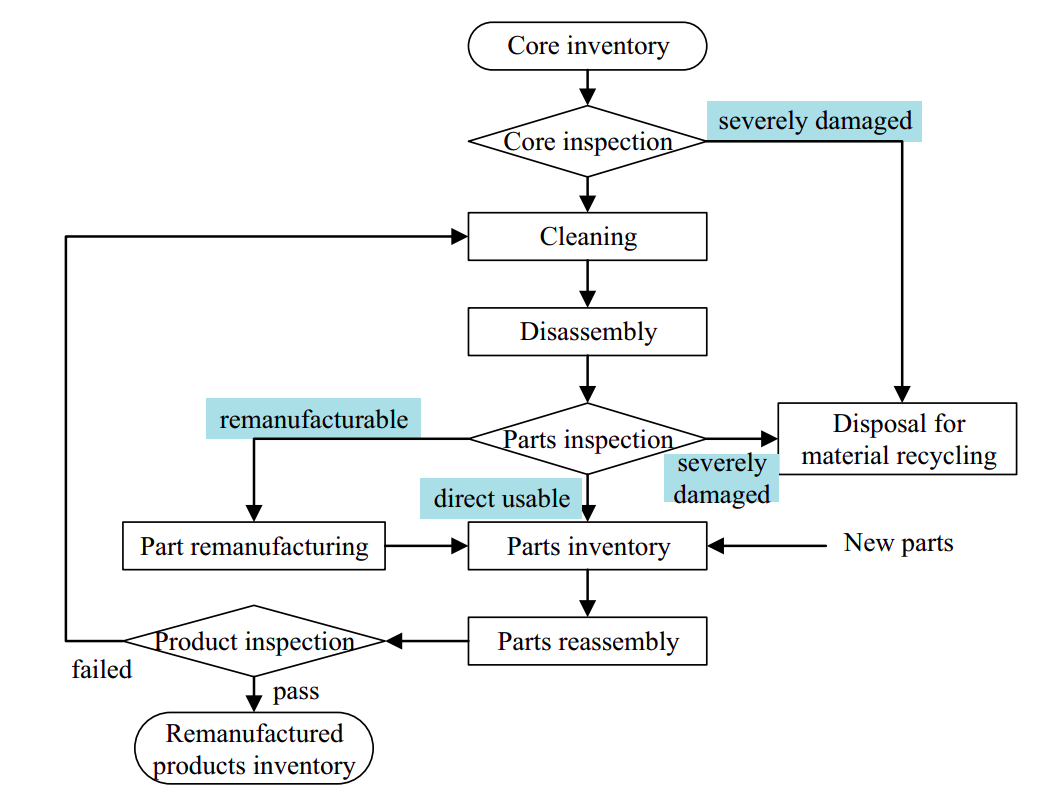
\includegraphics[width=\linewidth]{130quantification/internal/cei/zhao2021reman.png}
    \caption[An example of a generic remanufacturing process for vehicle components]{An example of a generic remanufacturing process for vehicle components~\cite{zhao2021reman}}
    \label{fig:remanufacturing}
\end{figure}
\FloatBarrier
\sectionEndlines
\clearpage


\subsubsection{Relevance of Remanufacturing and Refurbishing in FutuRaM's Waste Streams}

\wasteSubsubsecBATT
\begin{itemize}
    \item Electric Vehicle Batteries: Remanufacturing can involve replacing degraded cells or modules to extend their lifespan, thereby conserving lithium and cobalt.
    \item Laptop Batteries: Through remanufacturing, individual cells within the battery pack can be replaced or upgraded, enhancing the overall battery life and efficiency.
\end{itemize}

\wasteSubsubsecELV
\begin{itemize}
    \item Automotive Engines: Remanufacturing can include refurbishing engine components, such as pistons and bearings, to restore performance and efficiency.
    \item Transmission Systems: Rebuilding transmission systems with replaced or refurbished gears and bearings can significantly extend the life of the vehicle.
\end{itemize}

\wasteSubsubsecWEEE
\begin{itemize}
    \item Smartphones: Remanufacturing can involve replacing batteries, screens, and other components to restore them to like-new condition.
    \item Printers and Copiers: Components such as toner cartridges, drums, and fusers can be remanufactured to extend their service life and improve functionality.
\end{itemize}

\wasteSubsubsecCDW
\begin{itemize}
    \item Structural Steel Elements: In construction and demolition, steel beams and columns can be refurbished and reused in new construction projects.
    \item Wooden Beams and Flooring: Wooden elements can be remanufactured through processes like sanding, treating, and reinforcing for reuse in construction.
\end{itemize}


\sectionEndlines
\clearpage

\clearpage
\subsection{Remanufacturing: \textit{Scenarios}}

\boxws{This section will be filled out with the details of exactly how this parameter is incorporated into your stock and flow models}


\subsubsection{Global trends}


\subsubsection{Summary}

\boxreview{This summary will be compiled once the individual waste stream sections for each parameter are complete.}

\clearpage

\subsubsection[Scenario I: Business-as-usual]{\iconBAU Scenario I: Business-as-usual}

xx \\


\wasteSubsubsubsecBATT

\wasteSubsubsubsecCDW

\wasteSubsubsubsecELV

\wasteSubsubsubsecMIN

\wasteSubsubsubsecSLASH

\wasteSubsubsubsecWEEE

\subsectionEndline
\clearpage

\subsubsection[Scenario II: Recovery]{\iconREC Scenario II: Recovery}

xx \\


\wasteSubsubsubsecBATT

\wasteSubsubsubsecCDW

\wasteSubsubsubsecELV

\wasteSubsubsubsecMIN

\wasteSubsubsubsecSLASH

\wasteSubsubsubsecWEEE

\subsectionEndline
\clearpage


\subsubsection[Scenario III: Circularity]{\iconCIR Scenario III: Circularity}

xx \\


\wasteSubsubsubsecBATT

\wasteSubsubsubsecCDW

\wasteSubsubsubsecELV

\wasteSubsubsubsecMIN

\wasteSubsubsubsecSLASH

\wasteSubsubsubsecWEEE

\sectionEndlines
\clearpage
\clearpage

\subsection{The Sharing Economy: \textit{Description}}\cite{dabbous2021sharing, pwc2016sharing, dggrow2018sharing, dggrow2018sharingenv, dabbous2021sharing, ps2share2017sharing, zhu2021sharing}

\subsubsection{Definition}
The sharing economy is a socio-economic system that emphasizes the
collaborative sharing of goods and services via community-based online
platforms. It represents a shift from traditional ownership, where assets were
exclusively leased, to a flexible model allowing for both personal use and
lease. This flexibility is a hallmark of the sharing economy, which has grown
significantly in response to advancements in technology, such as e-commerce and
mobile connectivity, coupled with a societal push for more sustainable living
and efficient resource use.


\boxparameter{The sharing economy}{Stable}{Stable}{Strong increase}


\subsubsection{Context}
As the concept of ownership transforms, particularly among the younger
generation, the sharing economy has increasingly taken root in the EU market.
This shift towards more communal and cost-effective ways of accessing goods and
services is supported by a new wave of consumer behavior, underpinned by
technological innovation and a pressing need to reduce environmental waste and
resource duplication.

While the sharing economy is broad and its definition fluid, it is often
associated with collaborative consumption, though the two can differ in motives
and mechanisms. Collaborative consumption may span consumer-to-consumer and
business-to-consumer interactions, whereas the sharing economy typically
operates within the consumer-to-consumer sphere. The sharing economy is thereby
defined as an innovative marketplace where entities engage in the distribution
and utilization of products and resources, with scalability achieved through
technological means.

This socio-economic model has not only disrupted traditional business sectors
but has also brought new value to the global economy, with rapid and profound
market penetration. Financial forecasts have been bullish, with revenue for
sharing platform providers expected to increase from USD 18.6 billion in 2017
to an estimated USD 40.2 billion in 2022. Moreover, the overall value of the
global sharing economy is projected to expand significantly, from USD 14
billion in 2014 to USD 335 billion in 2025, reflecting an unprecedented growth
trajectory over a mere twelve years\cite{zhu2021sharing}. Such growth reflects
the substantial economic potential and transformative power of the sharing
economy in contemporary markets.

\subsubsection{Scope within the EU Economy}
The sharing economy has made a significant economic contribution to the EU,
with an estimated €26.5 billion added to the GDP in 2016~\cite{pwc2016sharing}.
This figure is expected to grow, indicating the sharing economy's increasing
importance within the EU's economic structure.

\subsubsection{Environmental Prospects}~\cite{dabbous2021sharing, pwc2016sharing, dggrow2018sharingenv}

See~\cite{zhu2021sharing} Table 2 for a summary of the studies on the
environmental impacts of the sharing economy.

The sharing economy has the potential to reshape consumption behaviors and
reduce environmental impacts by promoting the sustainable use of resources.
This economic paradigm encourages the efficient employment of underutilised
goods, which can lead to a decrease in the need for new products, thus
conserving resources and mitigating greenhouse gas emissions. It fosters a
lifestyle that lessens the adverse environmental effects of consumption while
improving quality of life.

Central to the sharing economy is the promotion of moderate consumption
patterns. This approach aims to reduce the excessive purchasing habits of
certain populations to alleviate ongoing environmental harm. The sharing
economy's alignment with green consumption practices encompasses waste
reduction, energy conservation, and the adoption of sustainable resources, all
while managing and moderating excessive consumption.

The impact on the fast fashion industry serves as a pertinent example, with the
sector's frequent turnover to keep pace with changing trends leading to
significant textile waste. Collaborative consumption through the sharing
economy can mitigate this waste by encouraging the reuse and extension of
clothing's service life. Clothing libraries are an example of how the sharing
economy can provide environmental benefits by prolonging the usable life of
garments.

Eco-efficiency is enhanced when environmental resources are utilised more
effectively, leading to an increased use of products with minimal environmental
burden. This is exemplified in collaborative fashion consumption, which could
reduce the prevalent overconsumption in the fashion industry. By facilitating
the exchange of underused clothing, the sharing economy can increase the
lifecycle of garments and encourage the production of more durable products.

Beyond the realm of fashion, car sharing and shared accommodation are other
aspects of the sharing economy with notable environmental benefits. Car sharing
can significantly reduce the number of vehicles needed, thereby lowering
exhaust emissions. Similarly, shared accommodations have been associated with
significantly lower carbon dioxide emissions compared to conventional hotel
stays.

However, the question of whether the sharing economy indeed delivers
environmental benefits remains contested.~\cite{zhu2021sharing,
  geissinger2019sharing} Detractors highlight the potential for an increase in
environmental burdens, particularly if the heightened usability of shared goods
escalates greenhouse gas emissions. The environmental and socio-economic
impacts engendered by the collaborative economy are intricate and highly
variable across different business models. Generally speaking, collaborative
consumption models that optimise the use of existing assets tend to exhibit a
lower environmental footprint compared to their traditional counterparts.
Nevertheless, there is a risk that the financial savings afforded by
collaborative consumption could spur additional spending and consumption, which
might negate the direct environmental savings. Despite such reservations, the
prevailing view is that the sharing economy, by transforming consumption from
ownership to communal use, can yield considerable environmental advantages.

\subsubsection{Implications for Waste Streams}

The adoption of sharing economy principles can influence various waste streams,
including:

\begin{itemize}
  \item \textbf{BATT (Waste Batteries):} As devices are shared and utilized more efficiently, the frequency of battery disposal could decline, mitigating the waste battery stream.
  \item \textbf{CDW (Construction and Demolition Waste):} The sharing of construction equipment and machinery could potentially slow down the turnover rate of these items, reducing associated waste.
  \item \textbf{WEEE (Waste Electrical and Electronic Equipment):} Sharing electronic devices extends their lifecycle and reduces the rate at which they are discarded, thereby impacting electronic waste volumes.
  \item \textbf{ELV (End-of-Life Vehicles):} A shift towards car-sharing services could reduce the demand for manufacturing new vehicles, potentially leading to a downturn in the generation of automotive waste.
\end{itemize}

The trajectory of the sharing economy indicates a shift towards collective
usage patterns. Its continuing evolution could play a critical role in the
future of critical raw material recovery systems by affecting demand and the
lifecycle of products, which, in turn, influences waste stream outputs. The
broader implications for the raw materials sector are significant, suggesting a
possible recalibration of recovery strategies for critical raw materials in
light of emerging consumption patterns.

\subsubsection{Challenges in Measuring Sharing Economy Growth}

Identifying a universal metric for the growth of the sharing economy is
challenging due to its diverse and dynamic nature. Current measures, such as
STOXX Global sharing economy indices, Solactive Sharing Economy Index and the
INDXX US Sharing Economy Index, largely revolve around the market sizes of
prominent sharing economy companies, such as Uber and Airbnb. These indices,
while useful, predominantly reflect the scalability of these businesses rather
than the sharing economy's broader impacts on production and waste reduction.

In the absence of a standardised metric, the assessment of the sharing
economy's expansion is often best approached through product-specific data.
This involves examining the adoption rates and usage trends of sharing services
at the product level to infer growth patterns. Such a detailed, product-centric
analysis allows for a closer inspection of the sharing economy's implications
on resource utilisation and waste generation, offering insights that aggregate
economic data may overlook.

\sectionEndlines
\clearpage
\clearpage
\subsection{The Sharing Economy: \textit{Scenarios}}

\boxws{This section will be filled out with the details of exactly how this parameter is incorporated into your stock and flow models}

\subsubsection{Summary}


\boxreview{This summary will be compiled once the individual waste stream sections for each parameter are complete.}

\clearpage

\subsubsection[Scenario I: Business-as-usual]{\iconBAU Scenario I: Business-as-usual}

xx \\


\wasteSubsubsubsecBATT

\wasteSubsubsubsecCDW

\wasteSubsubsubsecELV

\wasteSubsubsubsecMIN

\wasteSubsubsubsecSLASH

\wasteSubsubsubsecWEEE

\subsectionEndline
\clearpage

\subsubsection[Scenario II: Recovery]{\iconREC Scenario II: Recovery}

xx \\


\wasteSubsubsubsecBATT

\wasteSubsubsubsecCDW

\wasteSubsubsubsecELV

\wasteSubsubsubsecMIN

\wasteSubsubsubsecSLASH

\wasteSubsubsubsecWEEE

\subsectionEndline
\clearpage


\subsubsection[Scenario III: Circularity]{\iconCIR Scenario III: Circularity}

xx \\


\wasteSubsubsubsecBATT

\wasteSubsubsubsecCDW

\wasteSubsubsubsecELV

\wasteSubsubsubsecMIN

\wasteSubsubsubsecSLASH

\wasteSubsubsubsecWEEE

\sectionEndlines
\clearpage
\clearpage


\subsubsection{Conclusion}


\boxreview{This conclusion will be compiled once the individual waste stream sections for each parameter are complete.}


\sectionEndlines
\clearpage